\documentclass[Space3_Assign1.tex]{subfiles}

\begin{document}
\newpage
\section{Simulating Perturbations}

\subsection{Introduction}
The basic keperian model only accounted for an ideal two body system with no other effects when in reality, other forces act of the satellite. Compared to the gravitational motion between the Earth and the satellite however, these other effects are small. Therefore, they can be mathematically modelled as perturbations. While it is still an approximation, the error is reduced. Types of perturbations include;
\begin{itemize}
\item gravitational effects: such as the oblate Earth, third-body interactions such as the Moon, Sun or other planets
\item drag forces: from the Earth's atmosphere and from solar radiation pressure
\item unexpected thrusting: from malfunctioning thrusters
\end{itemize} 


\subsubsection{Earth oblateness}
For the standard simulation model in Question 1, it was assumed that the Earth was spherical. A perfectly spherical mass has an inverse square relation of the gravitational field to the force applied on a body. However, the Earth is slightly oblate, as it is flatter at the poles and wider at the equator than a sphere. 

Unlike using the keplerin model of Question 1, the classical orbital parameters change through time.

\subsubsection{Van Allen Probes}
Due to the highly elliptical orbit of the Van Allen Probes, most of the time the satellite is in MEO away from the Earth's atmosphere. As the inclination of the orbit keeps the satellite close to the equator, the perturbation due to the non-spherical earth 

Newtown's second law and his law of gravitation results in 
\begin{eqnarray}
\av{r}+\frac{\mu\dv{r}}{r^3} = a_p
\end{eqnarray}

\subsection{Methodology}
Equinoctial elements were used to remove the possible singularities that affect classical elements. The 



\subsection{Results/Discussion}
\begin{figure}[h]
\centering
\caption{Classical Elements over 12 days}
\label{fig:Q2classical_overtime}
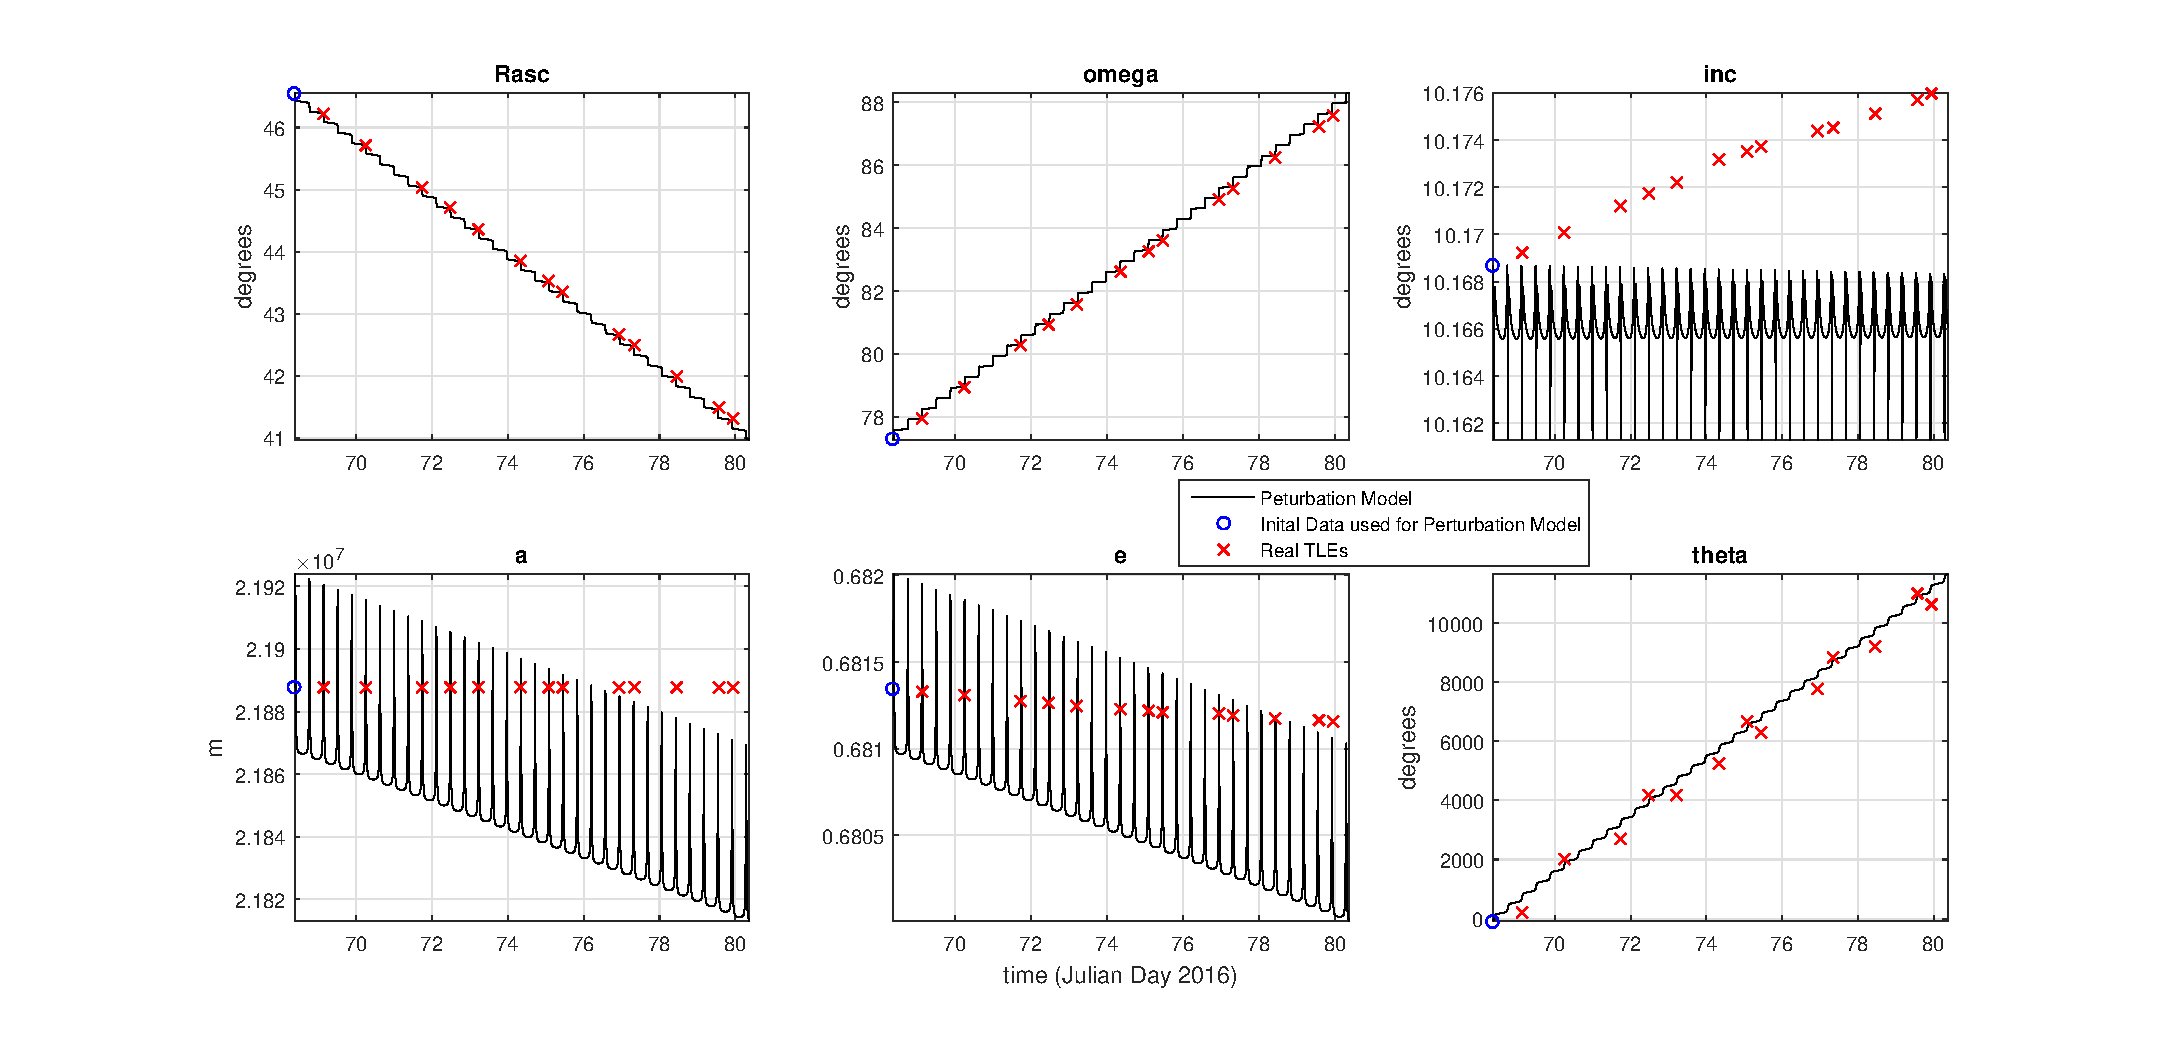
\includegraphics[trim = {4cm 0 3cm 0},clip,width=1\linewidth]{Q2classical_overtime.eps}
\end{figure}
\begin{figure}[h]
\centering
\caption{Equinoctial Elements over 12 days}
\label{fig:Q2equinoctial_overtime}
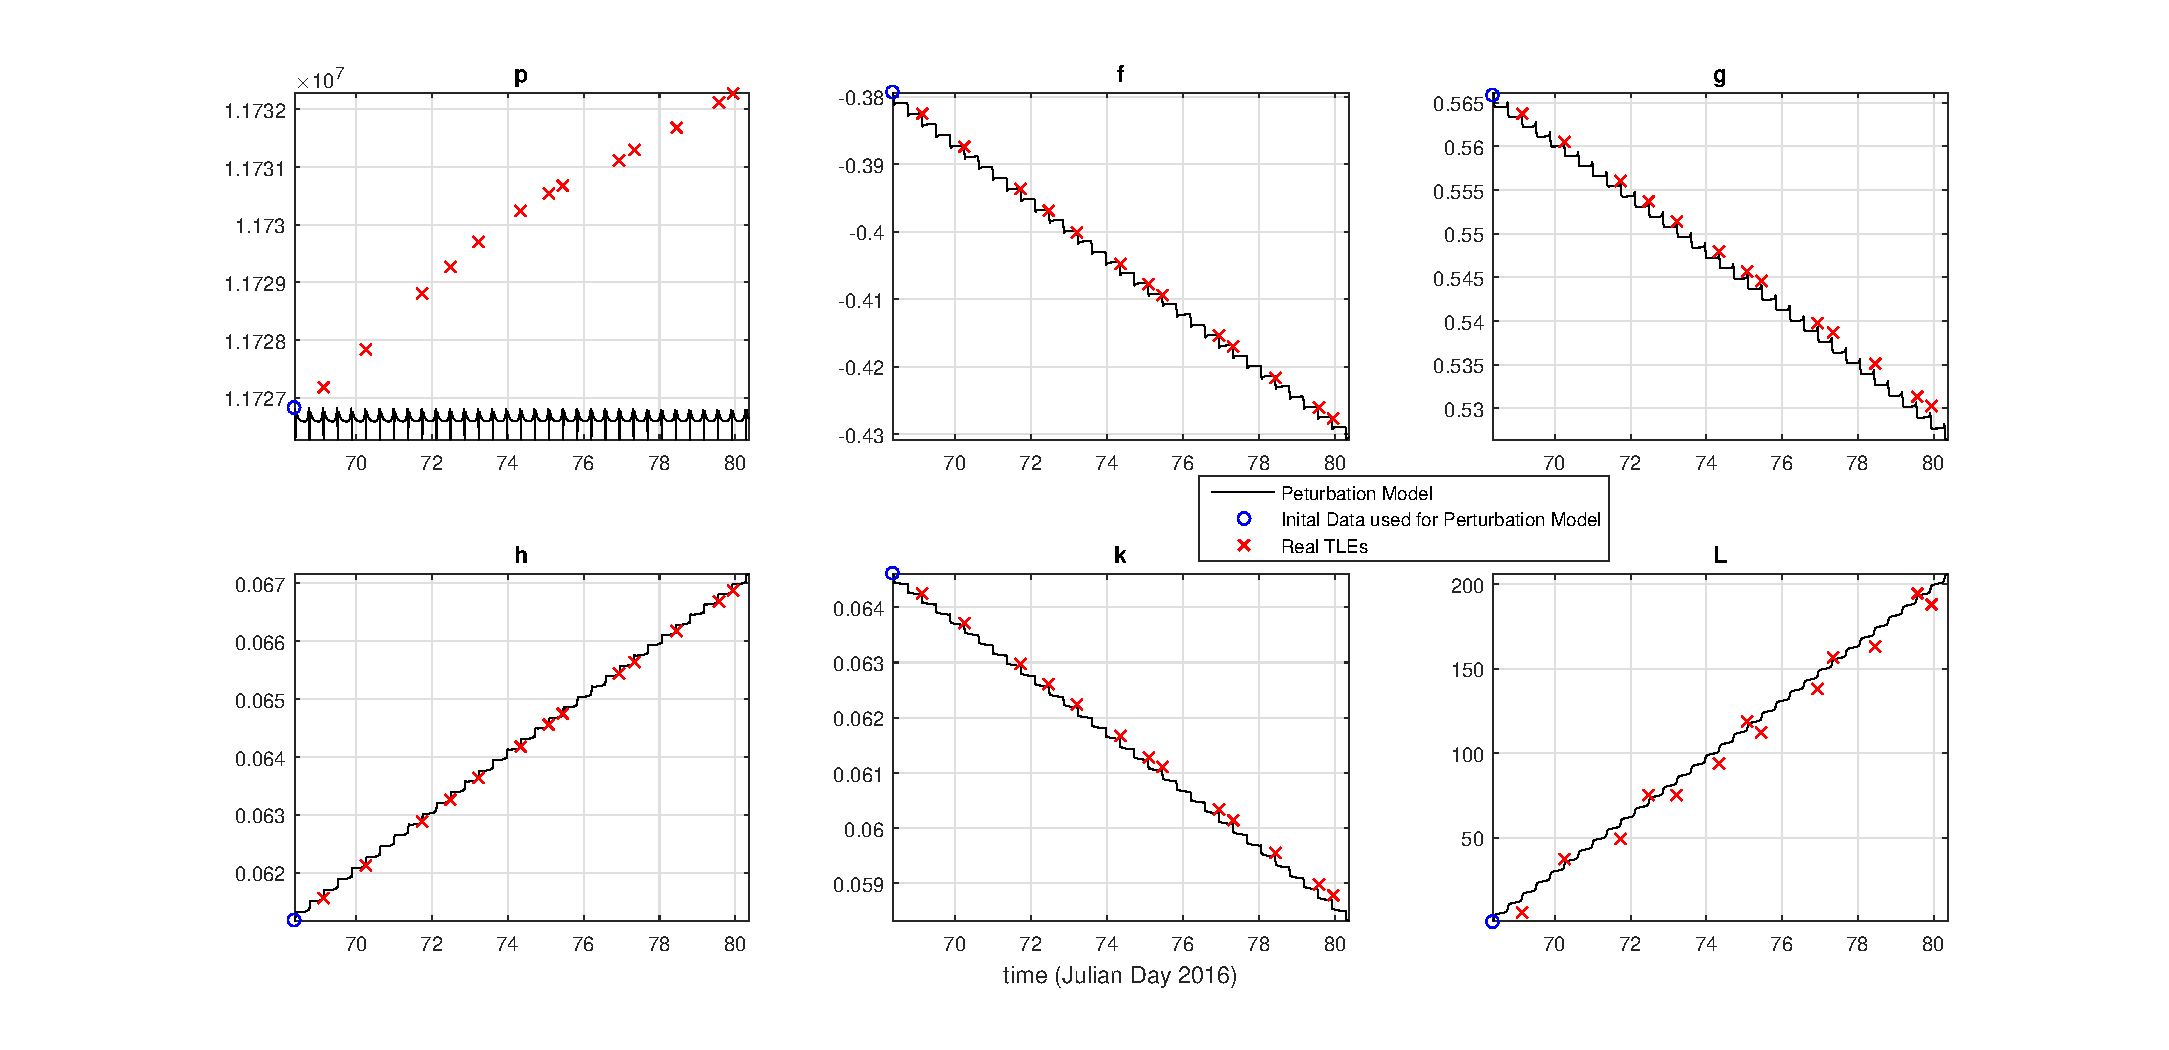
\includegraphics[trim = {4cm 0 3cm 0},clip,width=1\linewidth]{Q2equinoctial_overtime.eps}
\end{figure}



\end{document}